\section{Data Objects and Attribute Types}

\begin{frame}{Types of Data Sets}
	\begin{columns}
		\begin{column}{0.45\textwidth}
			\textbf{Records:}
			\begin{itemize}
				\item Relational records. \tikzmark{n1}
				\item Data matrix, e.g. numerical matrix, crosstabs.
				\item Document data: text documents, typically represented as
				      \textit{term-frequency vectors}.
				\item \textit{Transaction data}. \tikzmark{n2}
			\end{itemize}
			\textbf{Graph and network:}
			\begin{itemize}
				\item World wide web.
				\item Social information networks.
				\item Molecular structures.
			\end{itemize}
		\end{column}

		\begin{column}{0.45\textwidth}
			\vspace*{-0.7cm}
			\begin{table}
				\scalebox{0.8}{
					\begin{tabular}{|l|l|l|l|}
						\hline
						\textbf{Stud. ID.}    & \textbf{Forename} & \textbf{Surname} & \textbf{Study Programm} \\ \hline
						22305910              & Jane              & Doe              & Data Science            \\ \hline
						\tikzmark{t1}23061995 & Dominik           & Doe              & Informatics             \\ \hline
						23312331              & Friedrich         & Doe              & Data Science            \\ \hline
						20312131              & Melanie           & Doe              & Informatics             \\ \hline
					\end{tabular}
				}\\[1.5cm]
				\scalebox{0.8}{
					\begin{tabular} {|c|l|}
						\hline
						\textbf{TID}   & \textbf{Items}             \\
						\hline
						1              & Bread, Coke, Milk          \\\hline
						2              & Beer, Bread                \\\hline
						\tikzmark{t2}3 & Beer, Coke, Diapers, Milk  \\\hline
						4              & Beer, Bread, Diapers, Milk \\\hline
						5              & Coke, Diapers, Milk        \\
						\hline
					\end{tabular}
				}
			\end{table}
			\begin{tikzpicture}[remember picture,overlay]
				\draw[faugray,thick,->] ([yshift=1mm]n1) to[out=0,in=180] ([yshift=0mm, xshift=-0.5cm]t1);
				\draw[faugray,thick,->] ([yshift=1mm]n2) to[out=0,in=180] ([yshift=1mm, xshift=-0.5cm]t2);
			\end{tikzpicture}
		\end{column}
	\end{columns}
\end{frame}

\begin{frame}{Types of Data Sets}
	\begin{columns}
		\begin{column}{0.45\textwidth}
			\textbf{Ordered data:}
			\begin{itemize}
				\item Video data: sequences of images.
				\item Temporal data: time series. \tikzmark{n3}
				\item Sequential data: transaction sequences.
				\item Genetic sequence data.
			\end{itemize}
			\textbf{Spatial, image and multimedia:}
			\begin{itemize}
				\item Spatial data: maps.
				\item Image data. \tikzmark{n4}
				\item Video data.
			\end{itemize}
		\end{column}
		\begin{column}{0.45\textwidth}
			\vspace*{-0.5cm}
			\begin{center}
				\scalebox{0.8}{
					% Historical student numbers at FAU (Master Data Science)
					% Source: https://www.fau.de/files/2020/12/studierende_nach_lehreinheiten.pdf 
					% Last accessed: 09.04.2025
					\begin{tabular}{|c|c|c|c|c|c|c|c|}
						\hline
						\tikzmark{t3}\textbf{Semester} & WS22 & SS23 & WS23 & SS24 & WS24 \\ \hline
						\textbf{Students}              & 592  & 550  & 520  & 524  & 553  \\ \hline
					\end{tabular}
				} \\
				\vspace*{1.25cm}
				\scalebox{0.8}{
					% Fictional image of a university with dogs 
					% This is the next best thing to the previous TODO (picture of FAU)
					% as most images of the FAU are strictly copyrighted
					\tikzmark{t4}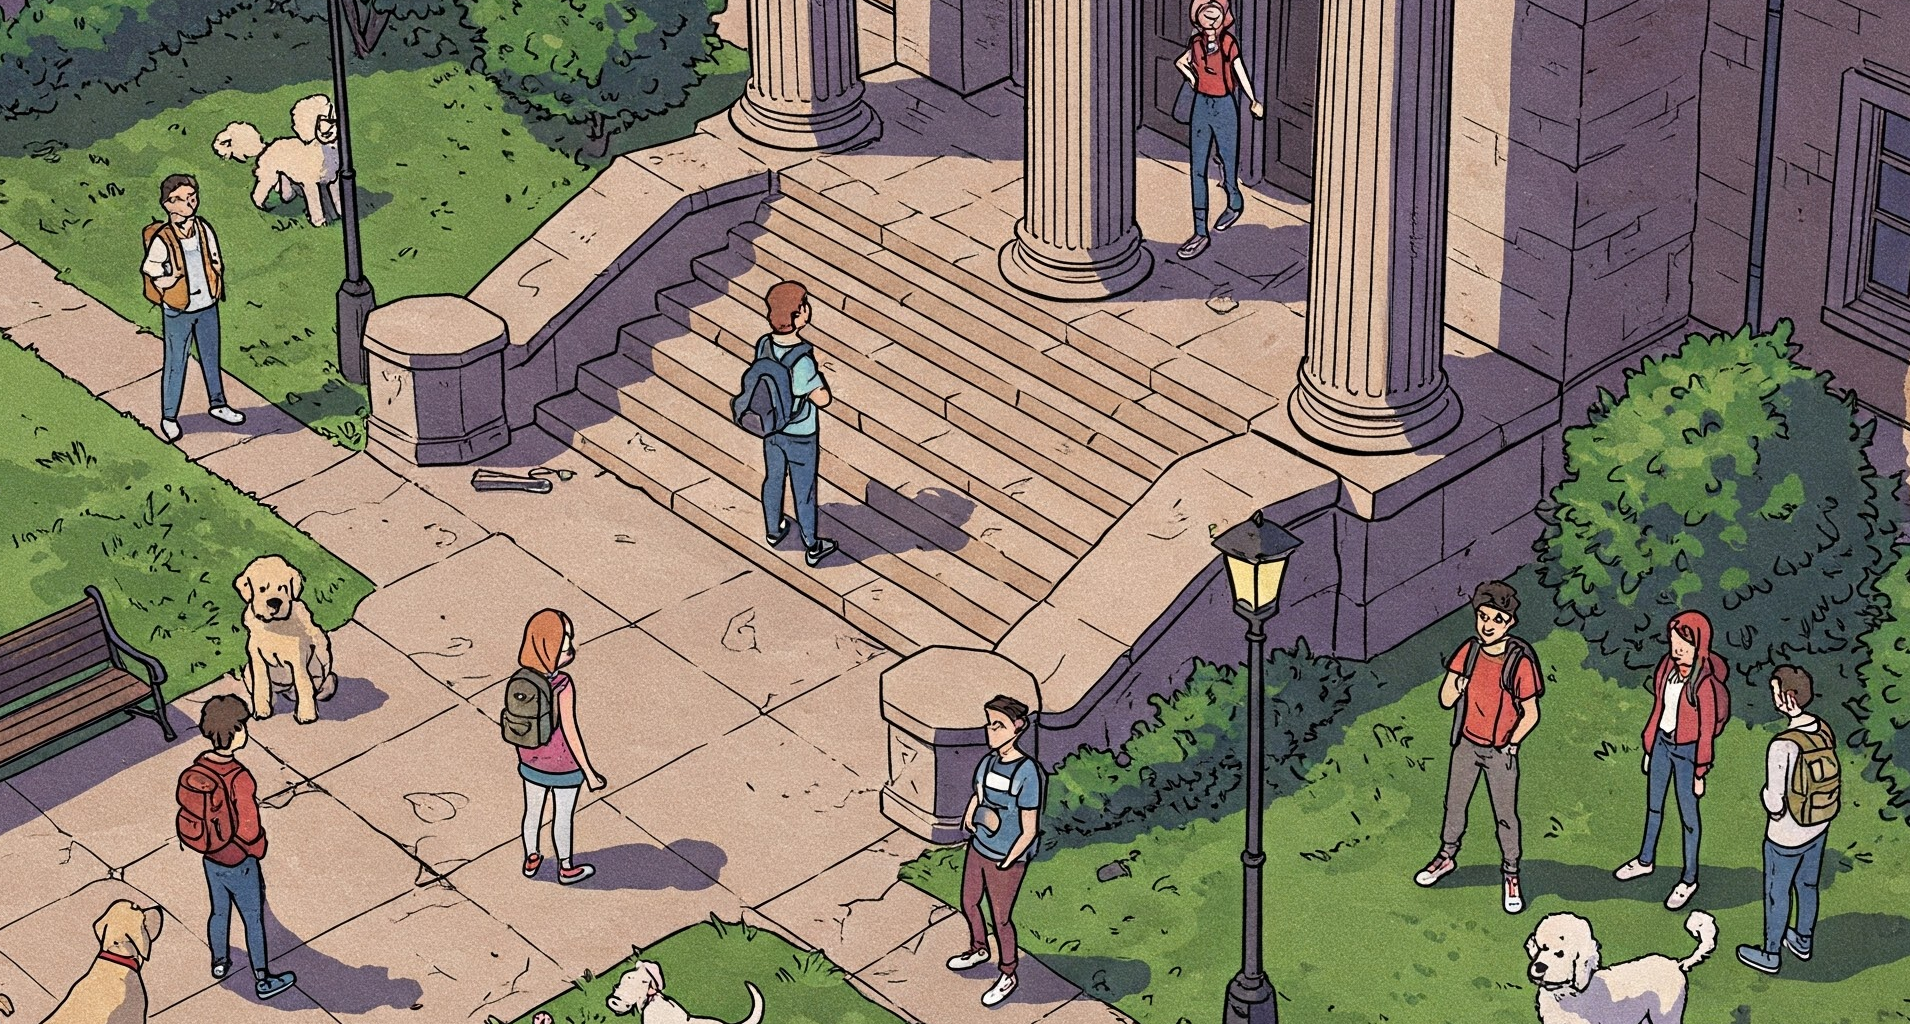
\includegraphics[width=0.95\textwidth]{img/university-with-dogs.png}
				}
			\end{center}
			\begin{tikzpicture}[remember picture,overlay]
				\draw[faugray,thick,->] ([yshift=1mm]n3) to[out=0,in=180] ([yshift=-2mm, xshift=-0.5cm]t3);
				\draw[faugray,thick,->] ([yshift=1mm]n4) to[out=0,in=180] ([yshift=1.4cm, xshift=-0.5cm]t4);
			\end{tikzpicture}
		\end{column}
	\end{columns}
\end{frame}

\begin{frame}{Important Characteristics of Structured Data}
	\textbf{Dimensionality}:\\
	Curse of dimensionality (sparse high-dimensional data spaces).\\[0.2cm]

	\textbf{Sparsity}:\\
	Only presence counts.\\[0.2cm]

	\textbf{Resolution}:\\
	Patterns depend on the scale.\\[0.2cm]

	\textbf{Distribution}:\\
	Centrality and dispersion.
\end{frame}

\begin{frame}{Data Objects}
	\begin{block}{Data Object}
		A data set consists of data objects. A single \textit{data object} represents an entity.
	\end{block}

	Also known as: Samples, examples, instances, data points, objects, tuples.\\\medskip

	Examples:
	\begin{itemize}
		\item Sales database: customers, store items, sales.
		\item Medical database: patients, treatments.
		\item University database: students, professors, courses.
	\end{itemize}

	\textbf{Data objects are described by attributes}:
	\begin{itemize}
		\item Database rows $\rightarrow$ data objects.
		\item Columns $\rightarrow$ attributes.
	\end{itemize}
\end{frame}

\begin{frame}{Attributes}
	\begin{block}{Attribute}
		An \textit{attribute} represents a specific characteristic such as customer
		unique identifier, customer name, and customer address.
	\end{block}

	Also known as: Variable, feature, field, dimension.\\\medskip

	\note[itemize]{
		\item \textit{dimension}: used in DWH, but also in statistics: number of
		observations not number of attributes/variables
		\item \textit{feature}: common in Machine Learning
		\item \textit{variable}: preferred by statisticians
	}

	Further terminology:

	\begin{itemize}
		\item \textit{Observations}: Observed or measured values of an attribute.
		\item An \textit{attribute vector} or \textit{feature vector} describes a
		      data object by its set of attributes.
		\item Data sets with one attribute are referred to as \textit{univariate}
		      (more than one: \textit{multivariate}).
	\end{itemize}

	\textbf{Two different views on attributes:}
	\begin{itemize}
		\item The view of the \textit{statistics} community.
		\item The view of the \textit{informatics} community.
	\end{itemize}
\end{frame}

\begin{frame}{Types of Attributes: Statistics}
	\begin{itemize}
		\item Most common classification based on Stevens\footnote{\fullcite{stevens1946}}:

	\end{itemize}
	\vspace*{1em}
	\begin{center}
		\scalebox{0.9}{
			\begin{tikzpicture}[
					every path/.style={
							thick,
							>=latex,
							rounded corners=5pt,
							draw,
							->
						},
					every edge/.style={draw, thick, >=latex},
					box/.style={
							draw,
							fill=white,
							rounded corners=.25em,
							% text height=.8em,
							outer sep=0,
							inner sep=.6em,
							align=center
						}
				]
				\node[box] at (0,0) (root) {Types of Measurements};
				\node[box, below left=2em and -3em of root] (qualitative) {Qualitative};
				\node[box, below right=2em and -3em of root] (quantitative) {Quantitative};

				\node[box, below left=2em and -2.5em of qualitative] (nominal) {Nominal};
				\node[box, below right=2em and -2.5em of qualitative] (ordinal) {Ordinal};

				\node[box, below left=2em and -2.5em of quantitative] (interval) {Interval};
				\node[box, below right=2em and -2.5em of quantitative] (ratio) {Ratio};

				\coordinate[below=1em of root.south] (root-below);
				\coordinate[above=1em of quantitative.north] (quantitative-above);
				\coordinate[above=1em of qualitative.north] (qualitative-above);
				\path[faugray] (root.south) -- (root-below) -- (qualitative-above) -- (qualitative.north);
				\path[faugray] (root.south) -- (root-below) -- (quantitative-above) -- (quantitative.north);

				\coordinate[below=1em of quantitative.south] (quantitative-below);
				\coordinate[above=1em of interval.north] (interval-above);
				\coordinate[above=1em of ratio.north] (ratio-above);
				\path[faugray] (quantitative.south) -- (quantitative-below) -- (interval-above) -- (interval.north);
				\path[faugray] (quantitative.south) -- (quantitative-below) -- (ratio-above) -- (ratio.north);

				\coordinate[below=1em of qualitative.south] (qualitative-below);
				\coordinate[above=1em of nominal.north] (nominal-above);
				\coordinate[above=1em of ordinal.north] (ordinal-above);
				\path[faugray] (qualitative.south) -- (qualitative-below) -- (nominal-above) -- (nominal.north);
				\path[faugray] (qualitative.south) -- (qualitative-below) -- (ordinal-above) -- (ordinal.north);
			\end{tikzpicture}
		}
	\end{center}
	\vspace*{1em}
	\begin{columns}
		\begin{column}{0.45\columnwidth}
			\centering
			\textbf{Qualitative Measurements:} \\
			Describes an attribute without providing a size or quantity.
		\end{column}
		\begin{column}{0.45\columnwidth}
			\centering
			\textbf{Quantitative Measurements:} \\
			Describes an objective, measurable attribute. Often numerical.
		\end{column}
	\end{columns}
\end{frame}



\begin{frame}{Qualitative Measurements}
	\begin{columns}[t]
		\begin{column}{0.45\columnwidth}
			\centering \textbf{Nominal Measurements:}
			\begin{itemize}
				\item Categories, states, or "names of things".
				\item E.g. \texttt{color} $= \{\text{blue,red,green}\}$.
				\item Other examples: \texttt{marital\_status}, \texttt{occupation}, \texttt{ID}, \texttt{ZIP code}.
				\item \textbf{Special case -} Binary measurements:
				      \begin{itemize}
					      \item Only two states ($0$ and $1$).
					      \item \textbf{Symmetric binaries}: both outcomes equally important, such as \texttt{sex}.
					      \item \textbf{Asymmetric binary}: outcomes not equally important. \\
					            E.g. medical test (positive vs. negative).\\
					            Convention: assign 1 to most important outcome (e.g. diabetes, HIV positive).
				      \end{itemize}
			\end{itemize}
		\end{column}
		\begin{column}{0.45\columnwidth}
			\centering \textbf{Ordinal Measurements}
			\begin{itemize}
				\item Values have a meaningful order (ranking), but magnitude between successive values is not known.
				\item E.g. \texttt{size} $= \{\text{small, medium, large}\}$
				\item Other examples: \texttt{grades}, \texttt{army rankings}.
			\end{itemize}
		\end{column}
	\end{columns}
\end{frame}

\begin{frame}{Quantitative Measurements}
	\begin{columns}[t]
		\begin{column}{0.45\columnwidth}
			\centering \textbf{Interval-Scaled Measurements}
			\begin{itemize}
				\item Measured on a scale of \textbf{equally sized} units.
				\item No true zero-point.
				\item Values have order.
				\item E.g. temperature in $^{\circ}C$ or $^{\circ}F$.
			\end{itemize}
		\end{column}
		\begin{column}{0.45\columnwidth}
			\centering \textbf{Ratio-Scaled Measurements}
			\begin{itemize}
				\item Inherent \textbf{zero point}.
				\item We can speak of values as being an order of magnitude larger
				      than the unit of measurement.
				\item E.g. temperature in Kelvin.
			\end{itemize}
		\end{column}
	\end{columns}

	\vspace*{2em}

	\begin{center}
		\begin{tikzpicture}[xscale=0.03]
			\def\Tzero{-273.15}  % absolute zero
			\def\Tnitro{-195.79} % liquid nitrogen
			\def\Tbody{36.8}     % body temperature
			\def\Tboil{100}      % boiling temperature
			\def\Tmax{140}       % maximum temperature on the scale
			\def\h{0.5}         % axis off sets
			\def\tick####1####2####3{\draw[thick,####3] (####1+.08) --++ (0,-.16) node[below=-.5pt,scale=1] {\scriptsize ####2};}
			\def\Ts####1{{25+50/(\Tmax-\Tzero)*(####1-\Tzero)}} % convert temperature to [25,50] range

			% AXIS
			\draw[->,thick] % degrees Celsius
			(1.02*\Tzero,0) -- (1.1*\Tmax,0) node[right] {$^\circ$C};
			\draw[->,thick] % Kelvin
			(1.02*\Tzero,-\h) -- (1.1*\Tmax,-\h) node[right] {K};
			\draw[->,thick] % Fahrenheit
			(1.02*\Tzero,-2*\h) -- (1.1*\Tmax,-2*\h) node[right] {$^\circ$F};

			% LABEL
			\node[above=-0.2em,align=center] at (\Tzero,0.1) {\scriptsize absolute\\[-2]\strut \scriptsize zero};
			\node[above=-0.2em,align=center] at (\Tnitro,0.1) {\scriptsize liquid\\[-2]\strut \scriptsize nitrogen};
			\node[left=4,above=-0.2em,align=center] at (0,0.1) {\scriptsize water\\[-2]\strut \scriptsize freezes};
			\node[right=4,above=-0.2em,align=center] at (\Tbody,0.1) {\scriptsize human\\[-2]\strut \scriptsize body};
			\node[above=-0.2em,align=center] at (\Tboil,0.1) {\scriptsize water\\[-2]\strut \scriptsize boils};

			% CELSIUS
			\tick{\Tzero,0}{$-273.15$}{faublue} % absolute zero
			\tick{\Tnitro,0}{\hspace{6pt}$-195.79$}{faublue} % liquid nitrogen
			\tick{0,0}{0}{faublue}              % freezing temperature
			\tick{\Tbody,0}{36.8}{faugreendark}            % body temperature
			\tick{\Tboil,0}{100}{faured}        % boiling temperature

			% KELVIN
			\tick{\Tzero,-\h}{0}{faublue}   % absolute zero
			\tick{\Tnitro,-\h}{77}{faublue}           % liquid nitrogen
			\tick{0,-\h}{273.15}{faublue}       % freezing temperature
			\tick{\Tbody,-\h}{310.0}{faugreendark}        % body temperature
			\tick{\Tboil,-\h}{373.15}{faured}   % boiling temperature

			% FAHRENHEIT
			\tick{\Tzero,-2*\h}{$-459.67$}{faublue} % absolute zero
			\tick{\Tnitro,-2*\h}{$-320$}{faublue}      % liquid nitrogen
			\tick{0,-2*\h}{32}{faublue}          % freezing temperature
			\tick{\Tbody,-2*\h}{98.2}{faugreendark}         % body temperature
			\tick{\Tboil,-2*\h}{212}{faured}     % boiling temperature
		\end{tikzpicture}
	\end{center}
\end{frame}

\begin{frame}{Types of Attributes: Informatics}
	\begin{itemize}
		\item The view of the \textit{informatics} community focuses on the \textbf{data
			      type} of the attribute:

	\end{itemize}
	\vspace*{1em}
	\begin{center}
		\scalebox{0.9}{
			\begin{tikzpicture}[
					every path/.style={
							thick,
							>=latex,
							rounded corners=5pt,
							draw,
							->
						},
					every edge/.style={draw, thick, >=latex},
					box/.style={
							draw,
							fill=white,
							rounded corners=.25em,
							% text height=.8em,
							outer sep=0,
							inner sep=.6em,
							align=center
						}
				]
				\node[box] at (0,0) (root) {Types of Attributes};
				\node[box, below left=2em and -2em of root] (categorical) {Categorical};
				\node[box, below right=2em and -2em of root] (numerical) {Numerical};
				\node[box, below left=2em and -2em of numerical] (continuous) {Continuous};
				\node[box, below right=2em and -2em of numerical] (discrete) {Discrete};

				\coordinate[below=1em of root.south] (root-below);
				\coordinate[above=1em of categorical.north] (categorical-above);
				\coordinate[above=1em of numerical.north] (numerical-above);
				\path[faugray] (root.south) -- (root-below) -- (categorical-above) -- (categorical.north);
				\path[faugray] (root.south) -- (root-below) -- (numerical-above) -- (numerical.north);

				\coordinate[below=1em of numerical.south] (numerical-below);
				\coordinate[above=1em of continuous.north] (continuous-above);
				\coordinate[above=1em of discrete.north] (discrete-above);
				\path[faugray] (numerical.south) -- (numerical-below) -- (continuous-above) -- (continuous.north);
				\path[faugray] (numerical.south) -- (numerical-below) -- (discrete-above) -- (discrete.north);
			\end{tikzpicture}
		}
	\end{center}
	\vspace*{1em}
	\begin{columns}
		\begin{column}{0.45\columnwidth}
			\centering
			\textbf{Categorical Attributes:} \\
			Corresponds to qualitative measurements. Most often strings.
		\end{column}
		\begin{column}{0.45\columnwidth}
			\centering
			\textbf{Numerical Attributes:} \\
			Corresponds to quantitative measurements. E.g. integers, floats.
		\end{column}
	\end{columns}
\end{frame}



\begin{frame}[c]{Numerical Attributes}
	\begin{columns}[t]
		\begin{column}{0.45\columnwidth}
			\centering \textbf{Continuous Attributes}
			\begin{itemize}
				\item Has real numbers as attribute values.\\
				      E.g. temperature, height, or weight.
				\item Practically, real values can only be measured and represented using a finite number of digits.
				\item Continuous attributes are typically represented as floating-point variables.
			\end{itemize}
		\end{column}
		\begin{column}{0.45\columnwidth}
			\centering \textbf{Discrete Attributes}
			\begin{itemize}
				\item Has finite or countably infinite elements.\\
				      E.g. ZIP code, profession, or the set of words in a collection of documents.
				\item Sometimes represented as integer variables.
				      % \item Note: Binary attributes are a special case of discrete attributes.
			\end{itemize}
			\begin{alertblock}{Note}
				Binary attributes are a special case of discrete attributes.
			\end{alertblock}
		\end{column}
	\end{columns}
\end{frame}
